\section{评估}
\label{sec:eval}

\nospacestitle{系统实现。 }
{\sys} 是一个既能服务传统模型、也能服务 LLM 的 {\maas} 系统，
共包含约 24,000 行 Rust 与 C++ 代码。
它建立在 Prefill/Decode 解耦、continuous batching 等广泛使用的 LLM 优化之上。
在实现过程中，
我们尽可能复用现有的高性能服务系统组件（这些组件本身不具备自动扩缩容能力）。
例如，
我们所有用于 LLM 的 GPU kernel 都来自 FlashInfer~\cite{flashinfer}。
我们之所以选择基于原生语言的实现框架，
是因为我们发现用 Python 实现细粒度调度比较困难。
更多实现细节见 \textsection{\ref{sec:appendix}}。

\begin{table}[!t]
    \centering
    \small{
        \resizebox{.97\linewidth}{!}{
            \ra{1.2}
            \begin{tabular}{lrr} \toprule
                                 & \textbf{集群 A} ($m$ x $g$) & \textbf{集群 B} ($m$ x $g$) \\ \hline
                GPU              & A800 80\,GB (4x8)   & A100 80\,GB (2x8) \\
                GPU-GPU（机内）  & 1.6\,Tbps NVLink    & 256\,Gbps PCIe    \\
                GPU-GPU（机间）  & 100\,Gbps RDMA      & 100\,Gbps RDMA    \\
                Host-GPU         & 128\,Gbps PCIe      & 128\,Gbps PCIe    \\
                SSD-GPU          & 10\,Gbps            & 10\,Gbps          \\ \bottomrule
            \end{tabular}
        }
    } \\[8pt]
    \begin{minipage}{1\linewidth}
        \caption{\small{\textit{
        评估所使用的集群。$m$ 表示主机数量，$g$ 表示每台主机上的 GPU 数量。
        }}}
    \label{tab:cluster}
    \end{minipage} \\[-10pt]
\end{table}


\stitle{测试平台。 }
我们的实验在表~\ref{tab:cluster} 所示的两个测试平台上完成。
得益于 NVLink，
集群 A 更适合服务需要张量并行的大模型（如 72\,B）；
而集群 B 则更适合服务单 GPU 模型。

\stitle{评测轨迹与模型。 }
由于扩缩需求与请求到达率密切相关，
我们选择了三类典型的真实世界轨迹：
BurstGPT~\cite{wang2024burstgpt}，以及来自 Azure 的 AzureCode 与 AzureConv~\cite{DBLP:conf/isca/PatelCZSGMB24}。
这些轨迹的详细形状展示在 {\fig{fig:eval-e2e}} 的第一列中。
由于这些轨迹来自服务能力不同的集群，
我们遵循标准做法~\cite{DBLP:conf/asplos/MiaoSDXL0J24,DBLP:journals/pvldb/AliPYS22,DBLP:conf/osdi/GujaratiKAHKVM20}，
利用 TraceUpscaler~\cite{traceupscaler} 在保持时间模式不变的前提下缩放轨迹，
使其平均请求率约为我们集群最大服务能力的一半。

在模型方面，
我们重点评估 LLM，
因为其他非 LLM 模型更小，使用 {\sys} 进行扩缩几乎是轻而易举的。
具体来说，
我们选择了 Llama3-8B、Mistral-24B 与 Qwen2.5-72B，
它们都是当前流行且精度较高的 LLM。
由于 {\sys} 对模型规模更为敏感，
为了简化描述，后文在不引起歧义的情况下直接使用参数规模来指代模型。
其中，8\,B 模型每个实例仅需 1 张 GPU，
而 72\,B 模型的单实例至少需要 4 张 GPU。

\stitle{对比对象。\,}
在未特别说明时，
我们将 {\sys} 与以下基线系统进行比较：
\begin{enumerate}[leftmargin=*]
    \itemsep0.5em
    \setlength{\itemindent}{0em}
    \item \textbf{\emph{ServerlessLLM (S-LLM)
    ~\cite{DBLP:journals/corr/abs-2401-14351}}}
    是当前最先进、以提升自动扩缩速度为重点的 {\maas} 系统。
    它使用主机内存缓存最近加载过的模型，并采用基于 time-to-live 的淘汰策略。
    当缓存未命中时，
    它会以尽量打满 SSD 带宽的方式从 SSD 加载参数。 \\[-15pt]

    \item \textbf{\emph{ServerlessLLM optimal (AllCache)}}
    是 ServerlessLLM 的理想化版本，
    它总是能够从主机缓存中加载参数，因此在扩缩速度上是 ServerlessLLM 的上界。 \\[-15pt]

    \item \textbf{\emph{DistServe}}~\cite{DBLP:conf/osdi/ZhongLCHZL0024}
    是当前最先进的、但不支持自动扩缩容的 LLM 服务系统。
    它采用 PD 解耦。
    我们选择它作为对比对象，
    是因为在 PD 解耦场景中，多实例扩缩（prefill 与 decode）以及避免扩缩干扰都更具挑战性。
    我们将在 \textsection{\ref{sec:eval-pd-colocation}} 中，再与常见的 PD 共置系统（如 vLLM~\cite{vllm}）进行比较。 \\[-15pt]
\end{enumerate}

\noindent
为了保证公平，
我们为 {\sys} 与 S-LLM 的各个变体使用相同的扩缩策略。

\subsection{真实轨迹下的自动扩缩性能}
\label{sec:eval-app}

\begin{figure*}[!t]
    \centering
    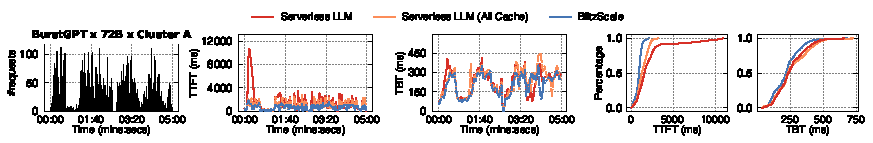
\includegraphics[width=1.01\textwidth,center]{./data/e2e-burstgpt.pdf} \\[0pt]
    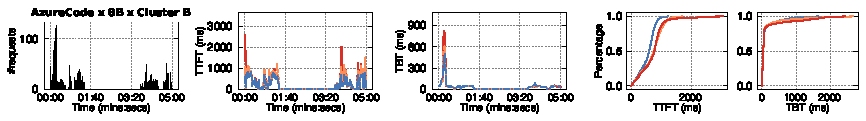
\includegraphics[width=1.01\textwidth,center]{./data/e2e-azurecode.pdf} \\[0pt]
    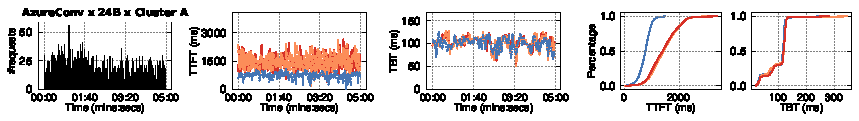
\includegraphics[width=1.01\textwidth,center]{./data/e2e-azureconv.pdf} \\[-5pt]
    \begin{minipage}{1\linewidth}
    \caption{\small{\textit{
        {\sys} 与 {\base} 在不同工作负载、模型与集群上的端到端性能对比。
    }}}
    \label{fig:eval-e2e}
    \end{minipage} \\[-10pt]
\end{figure*}

\noindent
受篇幅限制，
我们对每个模型只选择一个轨迹与一个集群进行展示。
{\fig{fig:eval-e2e}} 给出了在 prefill 与 decode 解耦、且两个阶段独立扩缩的设置下的端到端性能。
第一列展示轨迹的请求率，
第二列与第三列分别展示平均 TTFT 与平均 TBT，
其中每个点都是在 1 秒小时间窗内测得的平均时延；
最后两列则分别给出整个评测期间 TTFT 与 TBT 的累计分布函数（CDF）。
在本节中，
我们重点与 S-LLM 与 AllCache 比较；
由于 DistServe 不支持自动扩缩容，
我们将在下一小节单独与它比较。

\stitle{总体性能。 }
首先可以看到，
在所有工作负载上，{\sys} 的 TTFT 与 TBT 都是最低的，
这得益于其极快的自动扩缩速度。
具体而言，
在 BurstGPT 上，
{\sys} 的 TTFT 相比 S-LLM 与 AllCache 分别缩短了 75.5\,\% 与 21.1\,\%，
TBT 则分别缩短了 7.4\,\% 与 5.1\,\%。
不过，不同指标上的收益程度并不完全相同，
这是由 prefill 与 decode 阶段的不同特性共同决定的。
同时，
不同系统（尤其是 S-LLM）在不同工作负载下的行为也不一样，
这与它们的请求到达模式相关（见第一列）。
下面我们分别展开说明。

\stitle{TTFT 与 TBT 的差异。 }
在所有工作负载上，
{\sys} 对 TTFT 的改善都明显大于对 TBT 的改善。
这主要有两个原因。
第一，
借助我们优化后的策略（见 \textsection{\ref{sec:design-llm}}），
decode 实例可以被提前扩出，
而且我们对所有基线系统也采用了这一策略。
具体来说，
一旦 prefill 吞吐上升，
{\sys}（以及其基线）就会同步扩出 decode 实例，
因此在 decode 真正需要更多实例时，
扩缩时间已经与 prefill 阶段重叠，从而隐藏了一部分开销。
第二，
decode 的扩缩需求通常小于 prefill。
只要 decode 实例上的内存还足够，
所有系统通常都可以在几乎不产生排队的情况下处理 decode，
只是 TBT 会略有升高。
由于所有模型都采用了现代 LLM 优化中的 grouped-query attention~\cite{gqa}，
其显存占用较低，
因此 decode 侧通常比 prefill 侧更充裕。
尽管如此，
在三类工作负载上，{\sys} 的 TBT 相比 S-LLM 分别缩短了 5.1--7.4\,\%、88.3--94.1\,\% 与 0.7--1.8\,\%，
并且在各场景下也均优于 AllCache。

\stitle{不同工作负载之间结果差异。 }
借助高速网络扩缩与在线扩缩，
{\sys} 始终优于 AllCache；
但 S-LLM 相对 AllCache 的表现，则在不同工作负载之间有明显差异。
在 BurstGPT 上，
S-LLM 会在第一次突发（时间 0:05）出现显著 TTFT 尖峰，
但在之后的突发中与 AllCache 比较接近，
因为后续突发能够从主机缓存中获益。
相比之下，在 AzureCode 上，
S-LLM 在两次突发（时间 0:05 和 03:25）都会出现尖峰，
因为两次突发之间的间隔足够长，
导致主机缓存按照 TTL 策略被淘汰。
最后，在 AzureConv 上，
由于突发持续出现，S-LLM 基本总能命中主机缓存，
因此其性能——尤其从 CDF 图来看——与 AllCache 比较接近。

\subsection{性能与资源使用}
\label{sec:eval-resource}

\begin{figure*}[!t]
    \centering
    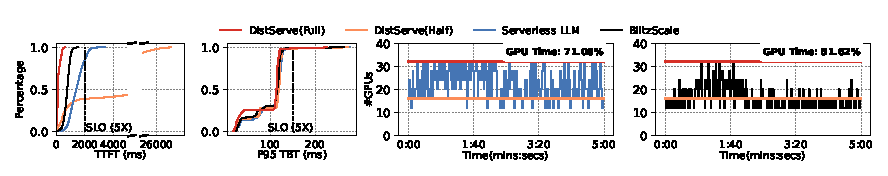
\includegraphics[width=1.01\textwidth,center]{./data/e2e-comparision-utilization-new.pdf}  \\[-10pt]
    \begin{minipage}{1\linewidth}
    \caption{\small{\textit{
        在 AzureConv 与 Mistral\,24B 组合下的 GPU 使用对比。
    }}}
    \label{fig:eval-e2e-gpu}
    \end{minipage} \\[-15pt]
\end{figure*}

\nospacestitle{与不支持自动扩缩容系统的比较。 }
我们首先将 {\sys} 与 DistServe 进行比较。
由于 DistServe 不支持自动扩缩容，
其性能高度依赖于预先分配的实例数量。
因此，我们评估两个设置：
DistServe (full) 使用整个集群的全部 GPU，
代表一种以浪费 GPU 为代价换取最佳性能的理想化配置；
DistServe (half) 则只使用在整个评测期间平均足以承载工作负载的实例数。
为简单起见，
这里我们只展示 AzureConv 上 24\,B 模型的结果，
整体趋势在其他设置中类似。
我们已经仔细校准了 DistServe 的性能，
确保在关闭 {\sys} 自动扩缩容后，
DistServe 与 {\sys} 在所有设置下表现一致。

{\fig{fig:eval-e2e-gpu}} 的前两列给出了时延结果。
首先可以看到，
DistServe (full) 的性能最好，
因为其 GPU 过度预配，不会遭受排队或扩缩开销。
尽管如此，
{\sys} 仍然在达到与 DistServe (full) 相同 SLO 的同时运行，
而 S-LLM 则有 18.7\,\% 的请求违反 SLO。
这里我们采用传统的 5\,$\times$ SLO~\cite{DBLP:conf/osdi/ZhongLCHZL0024}，
因为我们的工作负载（聊天与代码生成）都属于时延敏感型。
也就是说，
若某个请求的端到端 TTFT 或 TBT 超过平均时延的 5\,$\times$，
就视为违反 SLO。
最后，DistServe (half) 的性能最差：
平均来看，{\sys} 的 TTFT 与 TBT 分别比 DistServe (half) 短 95.8\,\% 与 1\,\%。
而做到这一点的同时，
{\sys} 用于服务该模型的 GPU 时间与 DistServe (half) 相同，
并且仅为 DistServe (full) 的一半。
下面我们进一步说明这一点。

\stitle{GPU 时间消耗。\,}
{\fig{fig:eval-e2e-gpu}} 的最后两列分别展示了 S-LLM 与 {\sys} 的 GPU 时间消耗。
对于 S-LLM 与 {\sys}，
我们分别收集每个时刻所有 prefill 与 decode 实例的聚合 GPU 使用量，
然后对曲线下方面积进行积分，得到整体 GPU 时间。
对于 DistServe 的两个变体，
其 GPU 时间在整个评测期间是常数。
结果表明，
得益于更快的自动扩缩速度，{\sys} 的 GPU 时间比 S-LLM 低 19.46\,\%。
当扩缩速度较慢时，
队列中会积压更多请求，
系统因而会触发更多扩缩动作，
最终消耗更多 GPU 时间。
而 {\sys} 则避免了这种额外消耗。
即便使用了更少的 GPU 时间，
{\sys} 的 TTFT 与 TBT 仍分别比 S-LLM 短 48.1\,\% 与 1.8\,\%。

\begin{figure}[!t]
    \centering
    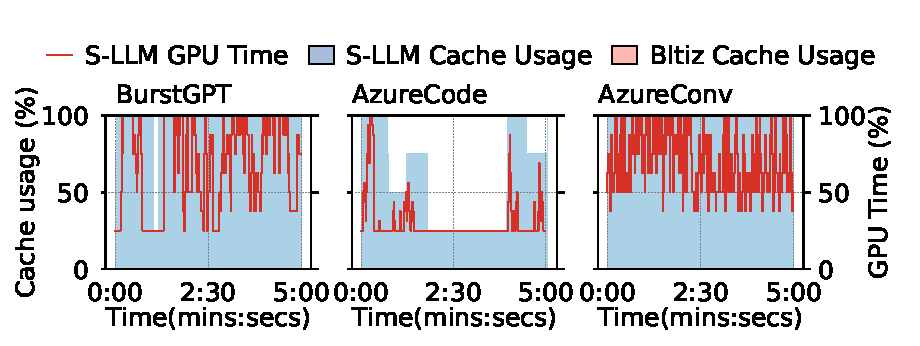
\includegraphics[width=1.0\linewidth,center]{./data/motiv-cache-usage-new.pdf}  \\[2pt]
    \begin{minipage}{1\linewidth}
    \caption{\small{\textit{
        在评测工作负载下，S-LLM 与 {\sys} 的主机缓存使用对比。
    }}}
    \label{fig:eval-cache-usage}
    \end{minipage} \\[-20pt]
\end{figure}

\stitle{主机缓存使用。\,}
与 ServerlessLLM 相比，
{\sys} 用于参数缓存的主机内存也更少。
{\fig{fig:eval-cache-usage}} 给出了不同系统的主机内存使用情况。
我们省略了 AllCache 与 DistServe：
前者始终会把参数完全复制到所有主机上，
后者则完全不需要缓存。
由于不同工作负载使用的集群不同，
我们对主机缓存使用量做了归一化。
这一结果传递了两个信息。
第一，{\sys} 仅需极少量的主机缓存（不到 1 份副本）就能实现快速自动扩缩容。
这与我们的设计一致：
我们优先从已经服务该模型的实例 GPU 上加载参数；
而即使当前没有任何服务实例，
借助基于网络的多播，我们也只需要 1 份主机缓存副本。
第二，ServerlessLLM 的内存使用与参与服务的主机数量成正比，
因此某个模型会迅速“污染”主机缓存。
对于一个同时服务很多模型、且主机缓存有限的 {\maas} 系统来说，
这种做法显然并不理想。

\subsection{更细粒度的性能分析}
\label{sec:eval-ablation}

\begin{figure*}[!t]
    \centering
    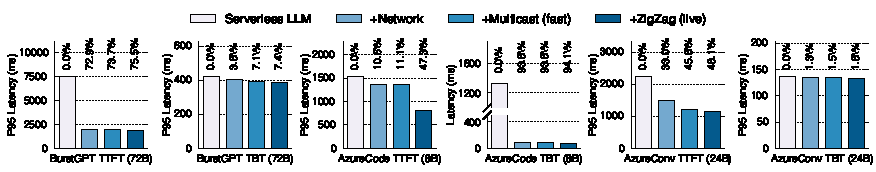
\includegraphics[width=1.01\textwidth,center]{./data/abl-new.pdf}  \\[-2pt]
    \begin{minipage}{1\linewidth}
    \caption{\small{\textit{
        对本文提出技术有效性的消融实验。
    }}}
    \label{fig:eval-alb}
    \end{minipage} \\[-20pt]
\end{figure*}

\begin{figure}[!t]
    \centering
    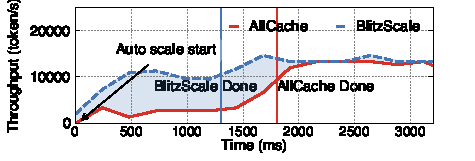
\includegraphics[width=1.0\linewidth,center]{./data/ext.pdf}  \\[2pt]
    \begin{minipage}{1\linewidth}
    \caption{\small{\textit{
        在集群 A 上把一个 24\,B 模型扩到 6 个 prefill 实例时，{\sys} 与 AllCache 的扩缩细节对比。
    }}}
    \label{fig:scale-breakdown}
    \end{minipage} \\[-5pt]
\end{figure}

\nospacestitle{在线扩缩的细节观察。 }
{\fig{fig:scale-breakdown}} 展示了使用 {\sys} 与 AllCache 把一个 24\,B prefill 模型扩到 6 个实例时的吞吐时间线。
{\sys} 使用了两条广播链（每条链覆盖 3 个实例），
其中链尾实例采用在线扩缩；
两条链的起始节点则是 decode 实例。
对于 AllCache，
它直接从新扩实例所在主机的内存中加载参数。
我们可以看到：
第一，哪怕只加载了很少的层（例如在 500\,ms 时），
{\sys} 也已经能够由于在线执行而逐步输出 token。
第二，借助基于 NVLink 的融合链路传输协议，
{\sys} 的扩缩速度甚至比 AllCache 更快：
它可在约 1,200\,ms 内完成扩缩，而 AllCache 约需 2,000\,ms。

\stitle{消融实验。 }
{\fig{fig:eval-alb}} 对我们提出技术的有效性进行了消融分析。
评估方式是逐步开启不同技术，并观察三种工作负载上的效果：
“+Network” 表示扩缩时使用高速计算网络而不是 SSD；
“+Multicast (fast)” 表示进一步采用 \textsection{\ref{sec:design-plan}} 中介绍的优化广播协议；
“+ZigZag (live)” 表示启用 \textsection{\ref{sec:design-pp}} 中的在线自动扩缩容机制。

首先可以看到，
所有技术都能提升端到端服务性能，
只是不同工作负载下收益大小不同。
“+Network” 在所有工作负载上都有效，
因为它为扩缩容数据平面提供了更高带宽。
“+Multicast (fast)” 在 AzureCode 与 AzureConv 上效果明显，
但在 BurstGPT 上收益较小，
这是因为受限于我们的集群规模，
在 72\,B 模型上最多只能同时扩 8 个实例，
因此几乎不存在“同时扩多个实例”的场景，
而这正是多播优化最擅长的场景。
在线自动扩缩容主要在 AzureCode 上最有效，
因为它是在网络更慢的集群 B 上评测的。
最后，
我们的方法在 decode 阶段上的收益通常不如 prefill 明显，
因为大多数情况下 decode 实例已经足够充足，
这一点我们已在 \textsection{\ref{sec:eval-app}} 中讨论过。
一个例外是 AzureCode：
在该工作负载中，prefill 吞吐增长得比其他负载更慢（见 {\fig{fig:eval-e2e}} 第一列），
因此 decode 实例的扩容会被更晚触发。
这使得 ServerlessLLM 的 SSD 慢扩缩无法被隐藏，
从而使更快的扩缩方式显得更有价值。

\begin{figure}[!t]
    \centering
    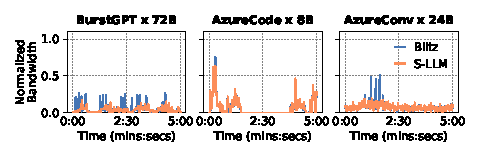
\includegraphics[width=1.0\linewidth,center]{./data/network-util.pdf}  \\[-10pt]
    \begin{minipage}{1\linewidth}
    \caption{\small{\textit{
        {\sys}（Blitz）的网络使用情况分析。
    }}}
    \label{ffig:eval-network-util}
    \end{minipage} \\[-10pt]
\end{figure}

\stitle{网络使用。 }
{\fig{ffig:eval-network-util}} 展示了 {\sys} 与 S-LLM 的网络使用情况。
可以看到，
尽管 {\sys} 利用计算网络执行自动扩缩，
而且扩缩频率也较高（见 {\fig{fig:eval-e2e-gpu}} 最后一列），
但其带来的额外网络开销仍然可以忽略不计。

\begin{figure}[!t]
    \centering
    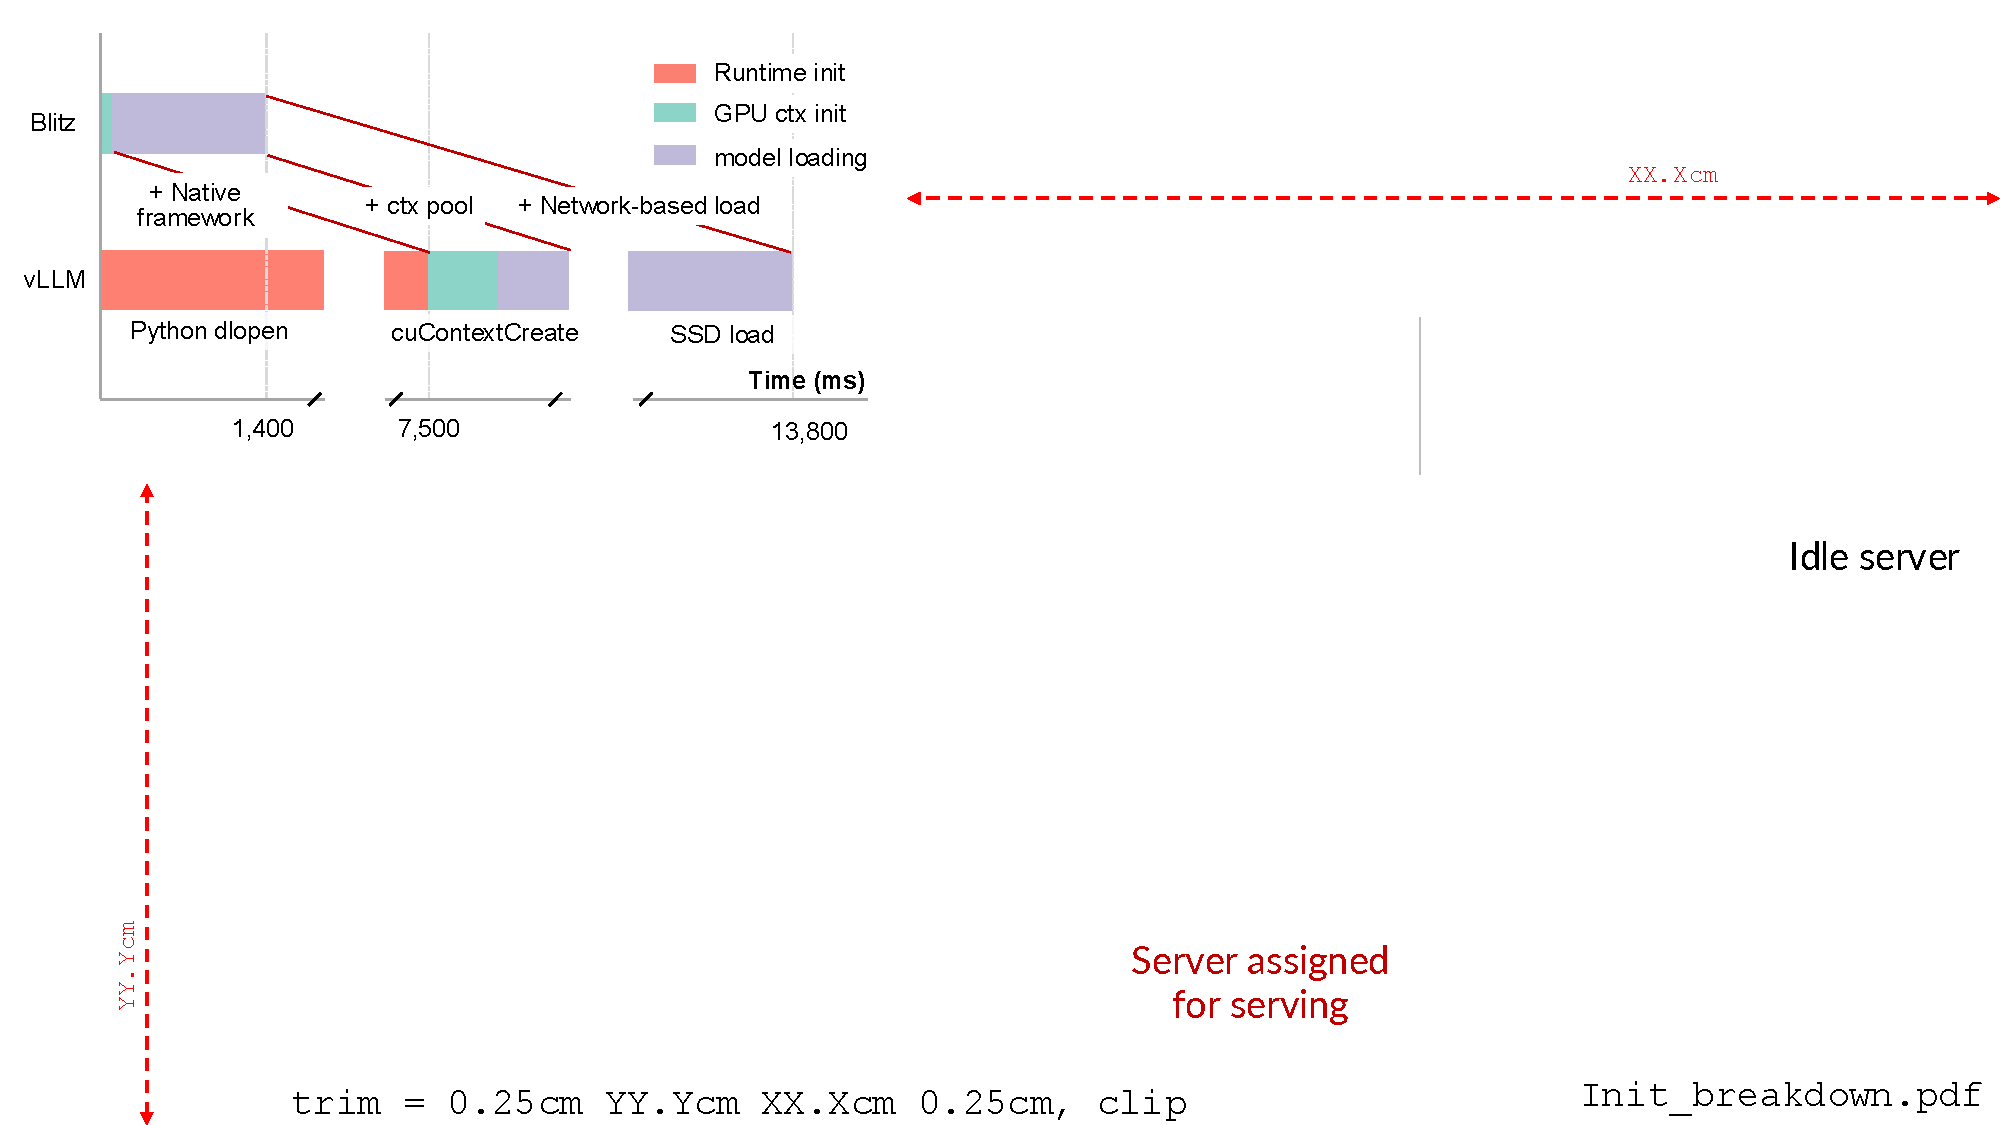
\includegraphics[width=.95\columnwidth, trim=0.25cm 10.9cm 18.55cm 0.9cm, clip]{figs/init_breakdown.pdf}
    \\[-8pt]
    \begin{minipage}{1\linewidth}
    \caption{\small{\textit{
        {\sys} 与 vLLM 的初始化时间对比。
    }}}
    \label{fig:breakdown}
    \end{minipage} \\[-10pt]
\end{figure}

\stitle{模型自动扩缩容中的控制平面与数据平面。 }
{\fig{fig:breakdown}} 将 {\sys} 与 vLLM 在自动扩缩时的控制平面和数据平面开销进行了对比。
结果表明，只要实现得当，
控制平面开销几乎可以忽略。

\subsection{LLM 的 PD 共置场景性能}
\label{sec:eval-pd-colocation}

\begin{figure}[!t]
    \centering
    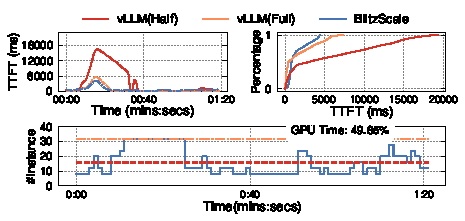
\includegraphics[width=1.0\linewidth,center]{./data/e2e-collocation-burstgpt.pdf}  \\[2pt]
    \begin{minipage}{1\linewidth}
    \caption{\small{\textit{
        {\sys} 与 vLLM 在 BurstGPT 工作负载上的对比。
    }}}
    \label{fig:eval-colocation}
    \end{minipage} \\[-10pt]
\end{figure}

\noindent
最后，{\fig{fig:eval-colocation}} 比较了 {\sys} 与 vLLM 在 PD 共置设置下的性能，
此时服务运行在 BurstGPT 工作负载与 Llama2-7B 模型上。
整体趋势与 PD 解耦场景类似：
{\sys} 的性能与过度预配的 vLLM 相当；
而与按平均需求预配的 vLLM 相比，
{\sys} 的 P99 TTFT 可缩短到其 0.24\,$\times$。
更有意思的是，
我们发现 {\sys} 的尾部 TTFT 甚至比过度预配的 vLLM 还更短，
这是因为我们的调度框架是针对集群级服务优化设计的。
